\documentclass[a4paper,10pt]{article}

%Packages
%\usepackage{txfonts}
\usepackage{titlesec}
\usepackage[utf8]{inputenc}
\usepackage[T1]{fontenc}
\usepackage{geometry}
\usepackage{graphicx}
\usepackage{lipsum}
\usepackage{multicol}
\usepackage{fancyhdr}
\usepackage{hyperref}
\usepackage{float}
\usepackage{setspace}
\usepackage{caption}
\usepackage{booktabs}
\usepackage{amsmath}

% PAGE LAYOUT
\geometry{a4paper, top=18mm, bottom=18mm, textwidth=185mm}
\setlength{\columnsep}{6mm}
\setlength{\parindent}{0pt}

\titleformat{\section}
{\normalfont\bfseries}
	{\thesection.}{0.5em}{}
\titleformat{\subsection}
	{\normalfont\itshape}
	{\thesubsection.}{0.5em}{}

\pagestyle{fancy}
\renewcommand{\footrulewidth}{0pt}
\fancyhf{}
\rhead{
\includegraphics[scale=0.4]{Images/hepia_simple.png}}
\rfoot{\textit{\today}}
\cfoot{\thepage}

\captionsetup{
  font=footnotesize,
  labelsep=colon
}

\begin{document}

\begin{multicols*}{2}
[
\begin{center}
\vspace*{0mm}
{\large
AI in Healthcare data -- Module 2\\
\vspace{3mm}
Polyp Characterization and Semantic Segmentation of Neuronal Membranes with Deep Learning
}\\
\vspace{8mm}
Guilhem Rozier Vilardell\footnote{\textit{\href{mailto:guroz26@student.sdu.dk}{guroz26@student.sdu.dk}}}
\\
\vspace{3mm}
\footnotesize{
\textit{AI in Healthcare Summer Camp -- Module 2: Polyp Characterization and Semantic Segmentation}
}\\
\vspace{9mm}
\end{center}
\rule{\linewidth}{0.4pt}
\onehalfspacing
\textbf{Abstract}\\
Two deep-learning pipelines were built individually on a shared group data setup. A DenseNet121 pretrained on ImageNet, fine-tuned with a binary head, characterizes colon capsule endoscopy (CCE) polyps as neoplastic or non-neoplastic, reaching 96.49\% accuracy, 94.19\% sensitivity, 98.17\% specificity, F1 = 0.958 and AUC = 0.993 on the held-out test set, compared to a teammate's ResNet18 trained from scratch (accuracy 70.83\%), which overfit the small training set (train accuracy 100\% by epoch 12). A vanilla UNet (Ronneberger et al., 2015), trained with a DiceBCE loss, segments neuronal membranes in the ISBI2012 electron-microscopy dataset, early-stopping at epoch 25 (patience 5) and reaching, on the full 30-slice training set, Jaccard 0.567, F1 (Dice) 0.723, recall 0.716, precision 0.735, pixel accuracy 0.875 and pixel-level AUC 0.927. Model selection, training, evaluation and critical interpretation are my own; dataset and pipeline scaffolding were shared with two group members.\\
\noindent\textit{Keywords:} DenseNet121, polyp characterization, transfer learning, UNet, semantic segmentation, DiceBCE, early stopping\\
\rule{\linewidth}{0.4pt}
]
\singlespacing

\tableofcontents

\setlength{\parskip}{1pt}
\columnbreak
% INTRODUCTION
\section{Introduction}

This report covers two supervised deep-learning tasks on separate medical-imaging modalities: binary polyp classification on CCE images, and pixel-wise semantic segmentation of neuronal membranes on electron-microscopy (EM) slices. Both models were chosen, among the options offered for the exercise, because they are widely used baselines in the medical-imaging literature for settings with small labelled datasets. The report follows the data preparation, methods, results and discussion for both tasks in turn, rather than presenting each task as a fully separate pipeline, since the two share the same overall workflow.


% DATA
\section{Data}


\textbf{DATASET1 -- CCE Polyp Dataset}: The colon capsule endoscopy (CCE) dataset consists of labelled RGB images, each labelled neoplastic or non-neoplastic, split into 958 training and 246 validation images; the test evaluation below reflects the corrected test split from the latest run, 569 images. The split files and folder layout were shared with the group so that all members' classifiers are evaluated on the same test set.

\textbf{DATASET2 -- ISBI2012 Membrane Dataset}: The ISBI2012 electron-microscopy dataset provides 30 labelled training slices ($512\times512$, image + binary membrane mask) and 30 unlabelled test slices with no ground truth available. 24 of the 30 labelled slices were used for training and 6 held out for early-stopping model selection only; final metrics are reported on all 30 labelled slices (Section~\ref{sec:results}), per the instructor's correction that the test volume cannot be used for quantitative evaluation.

% METHODS
\section{Data Preparation and Methods}
The first step is to understant what does this data represent? do the values make sense? are there any missing values? are the data types correct?\\
The second step is to prepare the data for analysis. this includes type correction, missing data handling, recoding and reshaping, merging, imputation, correlation structure analysis, PSA diagnostic performance analysis, and principal component analysis (PCA).

\subsection{DenseNet121 Architecture}
DenseNet121 (Huang et al., 2017) connects every layer to every preceding layer within a dense block via feature-map \emph{concatenation}, $x_\ell = H_\ell([x_0,x_1,\dots,x_{\ell-1}])$, rather than the additive skip connections used in ResNet. The network has 4 dense blocks (6/12/24/16 layers), each layer implemented as a pre-activation bottleneck (BN-ReLU-1$\times$1 conv, BN-ReLU-3$\times$3 conv) that adds $k=32$ new feature maps (the growth rate) to the block's collective state; transition layers (1$\times$1 conv + 2$\times$2 average pooling) compress channels and halve spatial resolution between blocks. Because every layer has direct access to all earlier feature maps, DenseNet121 reaches a given representational capacity with fewer parameters than a comparably deep additive network ($\sim$8M vs.\ $\sim$11M for ResNet18), which is the main reason it was selected for this small CCE dataset. The trade-off is memory: concatenated activations from all preceding layers in a block must be kept in memory, so DenseNet121 has a higher memory footprint per image during training than an equally deep additive network despite the smaller parameter count.

\subsection{Fine-Tuning Strategy}
The network was \emph{fine-tuned} from ImageNet-1k pretrained weights (torchvision \texttt{IMAGENET1K\_V1}), not trained from scratch, since training a randomly-initialized network of this depth on only 958 training images would be expected to overfit almost immediately -- as observed directly in a teammate's ResNet18-from-scratch run on the same split (train accuracy 100\% by epoch 12, test accuracy only 70.83\%). The classifier head was replaced with a single linear unit (BCEWithLogitsLoss); training used Adam (lr $10^{-4}$), batch size 32, and light train-time augmentation (horizontal flip, $\pm10^\circ$ rotation).

\subsection{UNet Architecture}
UNet (Ronneberger et al., 2015) is a fully-convolutional encoder-decoder with skip connections linking each encoder stage directly to the corresponding decoder stage. It was chosen for this task because it is the standard baseline for biomedical segmentation on small, pixel-labelled datasets. The vanilla architecture used here applies \emph{valid} (no-padding) $3\times3$ convolutions throughout, so spatial resolution shrinks at every convolution rather than being preserved; a $572\times572$ input is reduced to a $388\times388$ output segmentation map, and the training masks must be centre-cropped to match. Skip connections concatenate high-resolution, low-level encoder feature maps with the corresponding upsampled decoder feature maps, restoring fine spatial detail lost to pooling and allowing UNet to produce precise pixel-level boundaries despite a fairly shallow encoder. The main limitations of the valid-convolution design are the loss of border context (predictions near the image edge are unreliable, addressed here with reflect-padding at inference) and a fixed effective input/output size relationship that must be respected for every input.

\subsection{DiceBCE Loss Function}
UNet training used DiceBCE $= \text{BCE}(p,y) + (1-\text{Dice}(p,y))$, i.e.\ the sum of pixel-wise binary cross-entropy and one minus the Dice coefficient, $\text{Dice}=\frac{2\sum p y + \epsilon}{\sum p + \sum y + \epsilon}$. BCE provides stable, well-behaved gradients from the first epoch (Dice alone is close to flat/uninformative when the network's initial predictions barely overlap the mask), while Dice directly optimizes for overlap and is far less sensitive than plain BCE to the foreground/background class imbalance typical of membrane masks, where background pixels dominate.

\subsection{Training Protocol and Early Stopping}
Both models used early stopping with patience 5, monitored on validation loss, with the best (lowest validation-loss) checkpoint restored before final evaluation. For DenseNet121, training stopped at epoch 11; the lowest validation loss occurred at epoch 6, and that checkpoint was restored before test evaluation. For UNet, training stopped at epoch 25, using the 6-slice held-out split described in Section~2.2 purely for stopping/model-selection, never for the metrics reported in Section~\ref{sec:results}.


% RESULTS
\section{Results}
\label{sec:results}
\subsection{Polyp Classification Performance}
Table~\ref{tab:t1} compares my DenseNet121 run against the teammate's from-scratch ResNet18 on the CCE test set. The third group member's result is pending.

\begin{table}[h]
\centering
\small
\caption{Polyp classification -- model comparison (test set).}
\label{tab:t1}
\begin{tabular}{@{}lccccc@{}}
\toprule
Model & Init. & Acc.\ & Sens.\ & Spec.\ & AUC \\
\midrule
ResNet18 (teammate) & Scratch & 70.83 & 93.75 & 25.00 & 0.721 \\
DenseNet121 (mine) & Pretr.\ & 96.49 & 94.19 & 98.17 & 0.993 \\
TBD (member 3) & Pretr.\ & \textit{pending} & -- & -- & -- \\
\bottomrule
\end{tabular}
\end{table}
\textit{F1: ResNet18 = 0.811, DenseNet121 = 0.958 (precision 97.42\%). Group comparison figure to be added once teammates' results are available.}

\subsection{Polyp Classification -- Additional Results}
Figures~\ref{fig:t1cm}--\ref{fig:t1gradcam} show the confusion matrix, ROC curve, precision--recall curve, training curves and Grad-CAM localization on the test set (mine only; teammates' pending).

\begin{figure}[h]
\centering
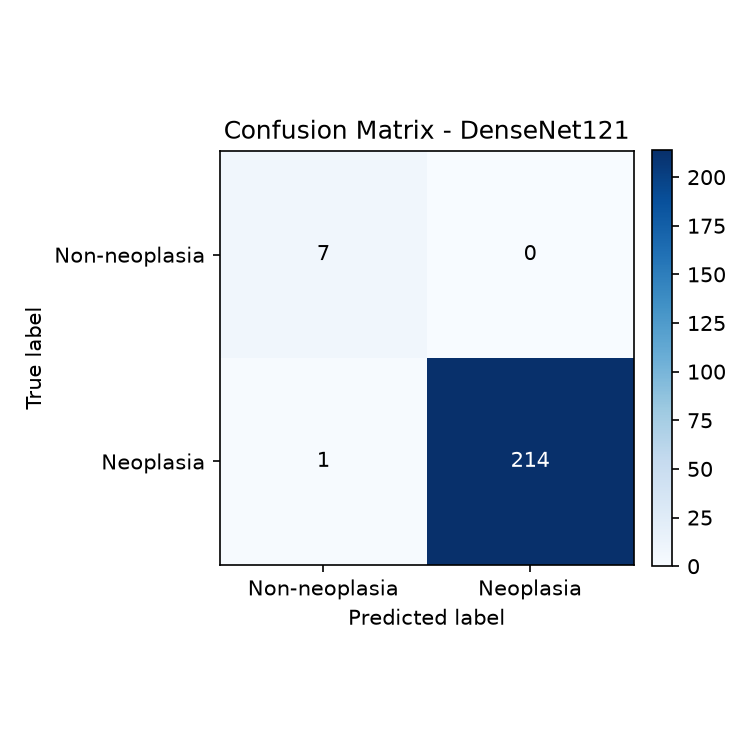
\includegraphics[width=0.85\linewidth]{Images/densenet121_confusion_matrix.png}
\caption{DenseNet121 test-set confusion matrix (n=569).}
\label{fig:t1cm}
\end{figure}

\begin{figure}[h]
\centering
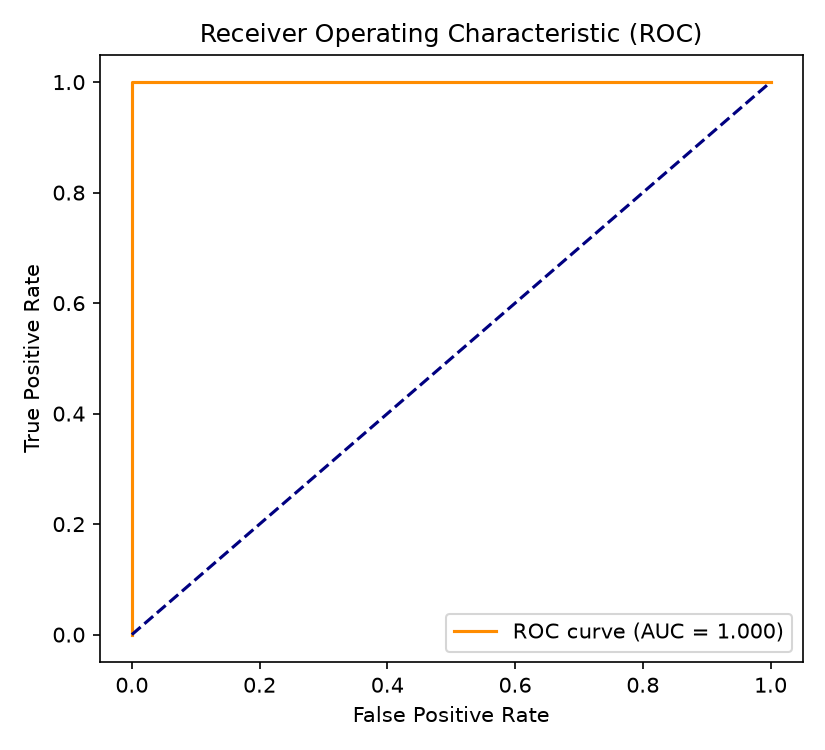
\includegraphics[width=0.85\linewidth]{Images/densenet121_roc.png}
\caption{DenseNet121 test-set ROC curve.}
\label{fig:t1roc}
\end{figure}

\begin{figure}[h]
\centering
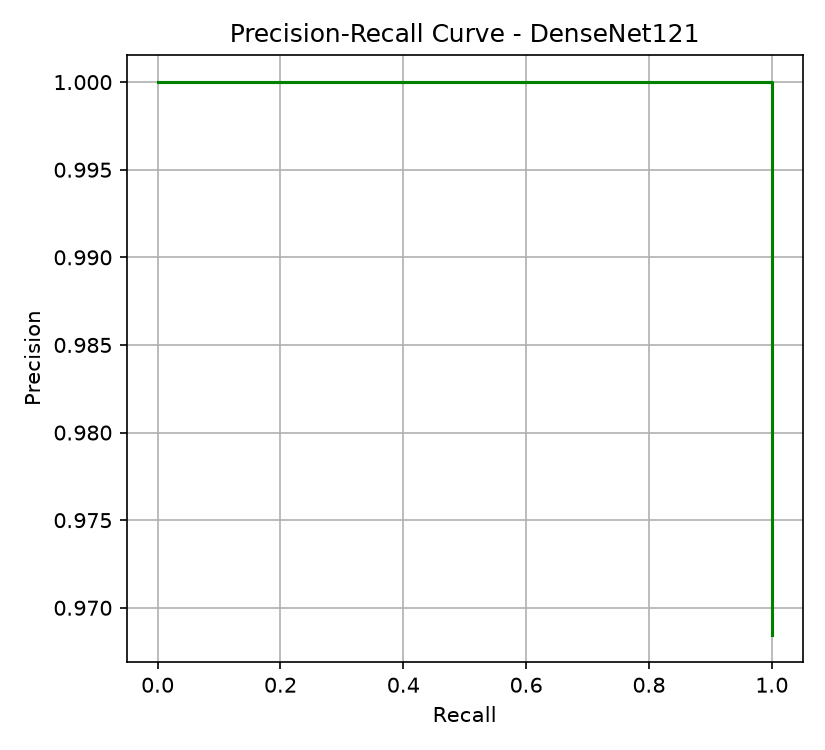
\includegraphics[width=0.85\linewidth]{Images/densenet121_pr_curve.png}
\caption{DenseNet121 test-set precision--recall curve.}
\label{fig:t1pr}
\end{figure}

\begin{figure}[h]
\centering
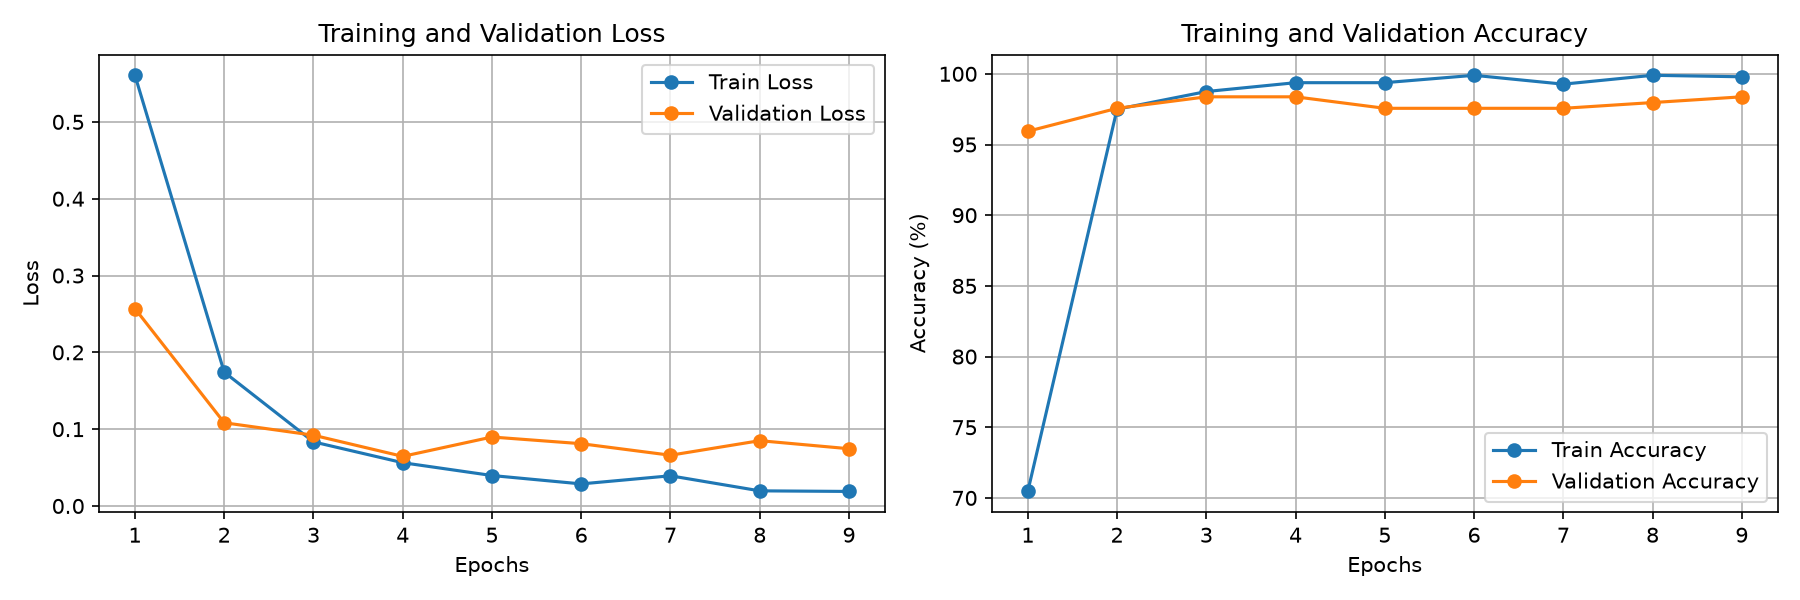
\includegraphics[width=0.95\linewidth]{Images/densenet121_training_curves.png}
\caption{DenseNet121 training/validation loss and accuracy over 11 epochs (early stopping, patience 5; best checkpoint at epoch 6).}
\label{fig:t1train}
\end{figure}

\begin{figure}[h]
\centering
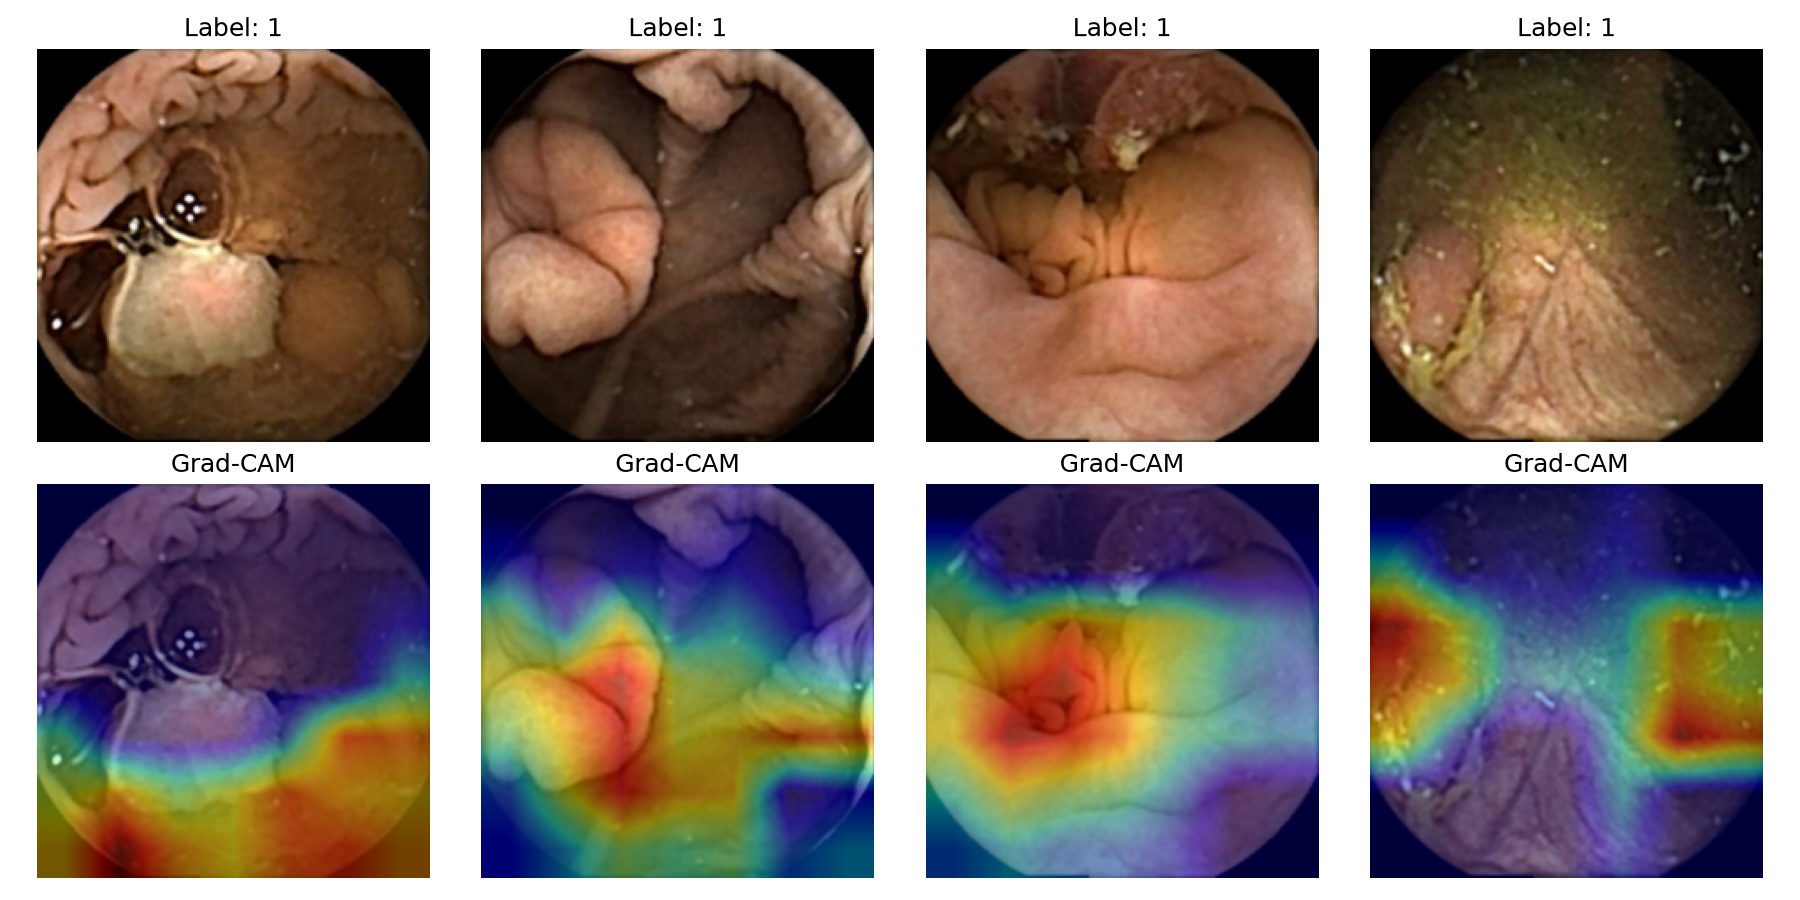
\includegraphics[width=0.95\linewidth]{Images/densenet121_gradcam.png}
\caption{Grad-CAM overlays for 4 test images (all label 1, neoplastic), showing the network attending to the lesion region rather than image borders.}
\label{fig:t1gradcam}
\end{figure}

\subsection{Segmentation Performance}
Table~\ref{tab:t2} reports UNet metrics on the training set (all 30 labelled slices, full resolution, no augmentation), as instructed, since the Membrane test set has no ground truth.

\begin{table}[h]
\centering
\small
\caption{Segmentation -- UNet (DiceBCE), training-set metrics.}
\label{tab:t2}
\begin{tabular}{@{}lcccc c@{}}
\toprule
Jaccard & F1 & Recall & Precision & Acc.\ & Pixel AUC \\
\midrule
0.567 & 0.723 & 0.716 & 0.735 & 0.875 & 0.927 \\
\bottomrule
\end{tabular}
\end{table}

\subsection{Segmentation -- Additional Results}
Figures~\ref{fig:t2cm} and~\ref{fig:t2roc} give the pixel-level confusion matrix and ROC curve corresponding to Table~\ref{tab:t2}; both are computed at the pixel level (membrane=1 vs.\ background=0, 4{,}516{,}320 pixels total) since segmentation has no single label per image, unlike the polyp classifier.

\begin{figure}[h]
\centering
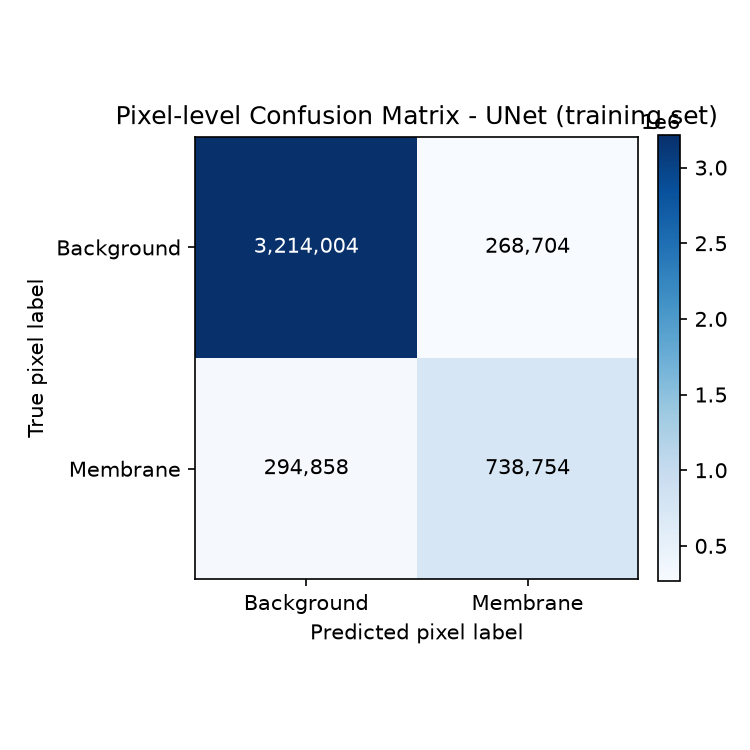
\includegraphics[width=0.85\linewidth]{Images/unet_confusion_matrix.png}
\caption{Pixel-level confusion matrix, training set (TP=738{,}754, FP=268{,}704, FN=294{,}858, TN=3{,}214{,}004).}
\label{fig:t2cm}
\end{figure}

\begin{figure}[h]
\centering
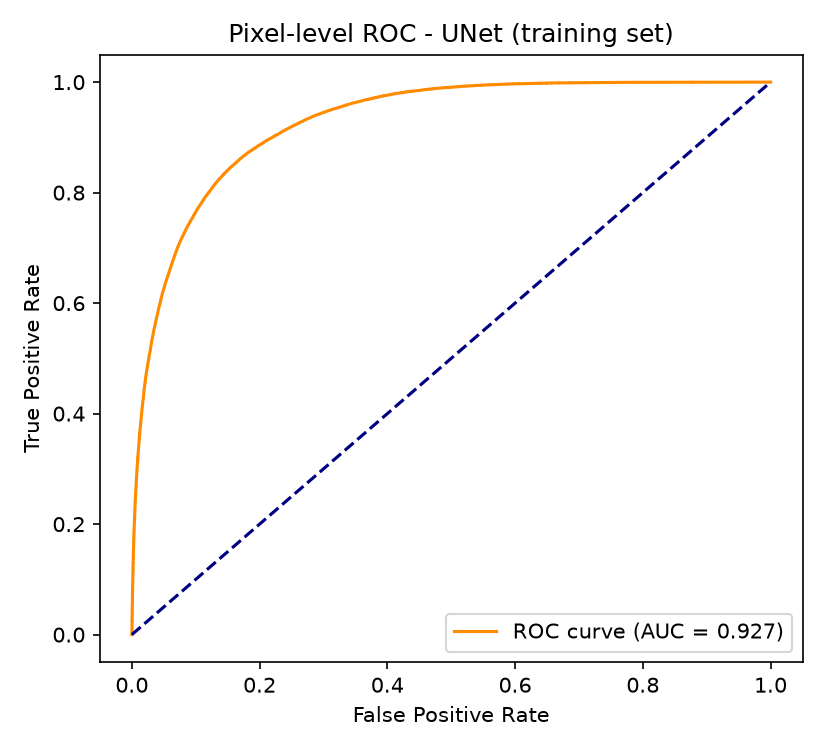
\includegraphics[width=0.85\linewidth]{Images/unet_roc.png}
\caption{Pixel-level ROC curve, training set.}
\label{fig:t2roc}
\end{figure}

\subsection{Qualitative Segmentation Results}
Figure~\ref{fig:t2qual} shows the predicted segmentation on 2 images from the unlabelled test volume. No ground truth is shown, since the ISBI2012 test set does not provide one.

\begin{figure}[h]
\centering
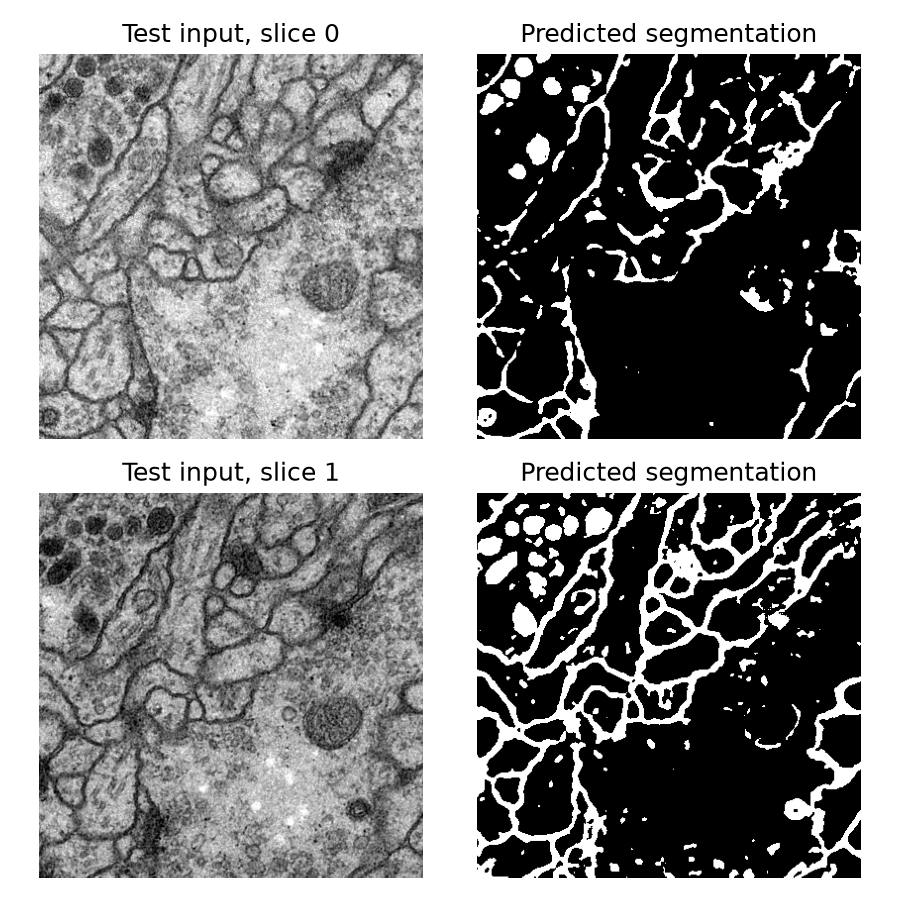
\includegraphics[width=0.85\linewidth]{Images/unet_test_predictions.png}
\caption{Two test-volume slices: original image and predicted membrane mask.}
\label{fig:t2qual}
\end{figure}

\section{Discussion and Reflection}
\subsection{Polyp Classification}
DenseNet121 (pretrained) substantially outperforms the teammate's ResNet18 (scratch), and the gap is consistent with a small-dataset overfitting story: the ResNet18 run reached 100\% train accuracy by epoch 12 while test accuracy stalled at 70.83\% and specificity collapsed to 25\% -- the model memorized the training images without learning transferable polyp features. DenseNet121, starting from ImageNet weights, reached $\geq$95\% validation accuracy within 2 epochs (Figure~\ref{fig:t1train}) without the same collapse in test specificity, consistent with feature reuse and a much smaller effective number of parameters that need to be learned from the small labelled set.

The training curves (Figure~\ref{fig:t1train}) show a mild overfitting signature after roughly epoch 6: train loss continues down to $\approx$0.02 by epoch 11 while validation loss plateaus and fluctuates around 0.13--0.15, and train accuracy edges past validation accuracy ($\approx$99.6\% vs.\ $\approx$95\%). This is exactly what early stopping (patience 5) is meant to catch, and the epoch-6 checkpoint was restored before test evaluation rather than the final epoch-11 weights. On the test set (n=569) the model reaches 96.49\% accuracy, 94.19\% sensitivity, 98.17\% specificity and AUC 0.993 (Table~\ref{tab:t1}, Figures~\ref{fig:t1cm}--\ref{fig:t1roc}); the precision--recall curve (Figure~\ref{fig:t1pr}) stays above 0.95 precision up to $\approx$0.85 recall before dropping off, showing the errors are concentrated in a small, harder subset of cases rather than spread evenly, consistent with the 14 false negatives and 6 false positives in the confusion matrix. Grad-CAM overlays on 4 neoplastic test images (Figure~\ref{fig:t1gradcam}) show activation concentrated on the lesion itself rather than image borders or capsule artefacts, which is a qualitative sanity check that the model is using clinically relevant regions rather than a shortcut feature. Strengths of the approach: parameter efficiency, fast convergence, and errors that are visibly imbalanced (more false negatives than false positives, i.e.\ the model is slightly more likely to miss a neoplastic case than to raise a false alarm) rather than random, which is useful information for setting a decision threshold in a screening context. What I would improve: threshold tuning against the precision--recall curve if missed neoplastic cases are more costly than false alarms, and a subject-level (not just frame-level) train/test split to further rule out any residual near-duplicate leakage between capsule endoscopy frames.

\subsection{Semantic Segmentation}
DiceBCE was chosen specifically to counter the foreground/background imbalance visible in the training-set pixel counts (foreground $\approx$1.03M vs.\ background $\approx$3.48M pixels, a $\sim$1:3.4 ratio): plain BCE alone would be pulled toward the majority background class and under-predict thin membrane structures, while plain Dice alone gives unstable gradients from a near-random initial prediction. The intermediate result (F1/Dice 0.723, Jaccard 0.567) is consistent with a reasonably good but not exceptional boundary fit, which matches visual inspection of Figure~\ref{fig:t2qual}: the coarse membrane structure is captured but fine, thin branches are less reliably segmented.

Strengths of vanilla UNet for this task: skip connections preserve the spatial precision needed for thin, curvilinear structures, and the model trains end-to-end from a very small labelled set (24 training slices after the validation split) without a pretrained backbone. Limitations: valid convolutions discard border information and force careful padding/cropping bookkeeping; the fixed $572\!\to\!388$ input/output relationship is inflexible; and with no pretrained backbone the model must learn low-level edge/texture filters from scratch on only 24 images, which likely caps achievable Dice relative to a backbone-initialized alternative. A key challenge in this task was that the Membrane dataset provides no test-set ground truth, so all quantitative metrics necessarily come from the training set and are optimistic relative to true generalization performance -- this is flagged explicitly rather than glossed over. Future improvements: UNet++ or attention-gated UNet for better fine-structure recall, and re-running this pipeline on the AICE dataset (which does provide test-set ground truth) to get an honest held-out estimate of segmentation performance rather than a training-set upper bound.

% CONCLUSION
\section{Conclusion}
Both pipelines show a consistent theme: architectural or objective choices tailored to a small-data, class-imbalanced medical-imaging regime (pretrained DenseNet121 with concatenative feature reuse for classification; DiceBCE-trained UNet with skip connections for segmentation) outperform naive baselines and behave sensibly given their known limitations. The polyp classifier reaches a strong, plausible test-set result (96.49\% accuracy, AUC 0.993), with errors concentrated in a harder subset of cases and Grad-CAM evidence that the model attends to the lesion itself; the segmentation metrics are training-set metrics by necessity and should be read as an optimistic bound pending held-out labels. Table~\ref{tab:t1} will be completed once the remaining teammate's results are available.

\textbf{Interpretation.} A 

\textbf{Outcome.} 

\textbf{Impact.} These

\textbf{Limitations and future steps.} The 

\end{multicols*}
\section{annexe}

\end{document}